\documentclass[a4paper, 12pt]{report}

%%%%%%%%%%%%
% Packages %
%%%%%%%%%%%%

\usepackage[spanish]{babel}
\usepackage{packages/sleek}
\usepackage{packages/sleek-title}
\usepackage{packages/sleek-theorems}
\usepackage{packages/sleek-listings}
\usepackage{dirtree}
\usepackage{graphicx}
\usepackage{caption}
\usepackage{subcaption}

%%%%%%%%%%%%%%
% Title-page %
%%%%%%%%%%%%%%

\logo{./resources/pdf/logo.pdf}
\institute{Universidad Politécnica de Cartagena}
\faculty{Ingeniería Telemática}
%\department{Department of Anything but Psychology}
\title{Aplicaciones en Internet}
\subtitle{Web de recomendación de películas}
\author{\textit{Autores}\\\textsc{Álvaro Herández Riquelme}\\ y \textsc{André Yermak Naumenko}}
%\supervisor{Linus \textsc{Torvalds}}
%\context{A long time ago in a galaxy far, far away...}
\date{\today}

%%%%%%%%%%%%%%%%
% Bibliography %
%%%%%%%%%%%%%%%%

\addbibresource{./resources/bib/references.bib}

%%%%%%%%%%
% Macros %
%%%%%%%%%%

\def\tbs{\textbackslash}

%%%%%%%%%%%%
% Document %
%%%%%%%%%%%%

\begin{document}
    \maketitle
    \romantableofcontents



    \newpage
    \newpage

    \chapter{Introducción}
    Este documento tiene como objetivo explicar el funcionamiento de la aplicación web de recomendación de películas llamada \texttt{El Recomendador}.

    El proyecto incluye funcionalidades clave como la autenticación de usuarios, gestión de perfiles, un catálogo dinámico de películas, un sistema de puntuación y comentarios, y algoritmos avanzados para la recomendación y el ranking de películas. Además, se ha diseñado una interfaz intuitiva y una arquitectura robusta basada en PHP, JavaScript, MATLAB y SQL.

    Cada capítulo abordará las distintas funcionalidades y aspectos técnicos del proyecto de forma sintética y clara para poder así comprender el funcionamiento al completo de la aplicación.

    \section{Perfil de labit601}

    Nuestro usuario será el \textbf{ai9} de los servidores de la UPCT, y la contraseña será \textbf{ai2025}. Todo el código está en la carpeta publica \textbf{public\_html}. También se puede comprobar el funcionamiento de la web en su enlace correspondiente.
    \chapter{Index}

    En primera instancia, el usuario accederá a esta página. En ella, el usuario se puede encontrar una portada con una breve descripción de la web, y en ella va incluida dos formularios, una de registro y otra de inicio de sesión. Se ha optado por una portada simple y minimalista para que el usuario pueda acceder rápidamente a la web.
    \section{index.html}

    A nivel técnico, la página principal se compone de un formulario de inicio de sesión y un formulario de registro. Ambos formularios están diseñados como una extensión HTML del archivo \textit{index.html} de tal modo que son gestionadas por separado y se pueden encontrar en los directorios \textit{/auth/register.php y /auth/registerform.html} para el registro y \textit{/auth/login.php y /auth/loginform.html} para el inicio de sesión.

    Para el fondo hemos elegido una animación discreta de una luz recorriendo la pantalla, esto se puede asemejar a los salvapantallas de los televisores con el logo DVD que cuando chocan con un borde, cambia su camino.

    \begin{figure}[h!]
        \centering
        \begin{subfigure}{0.45\textwidth}
            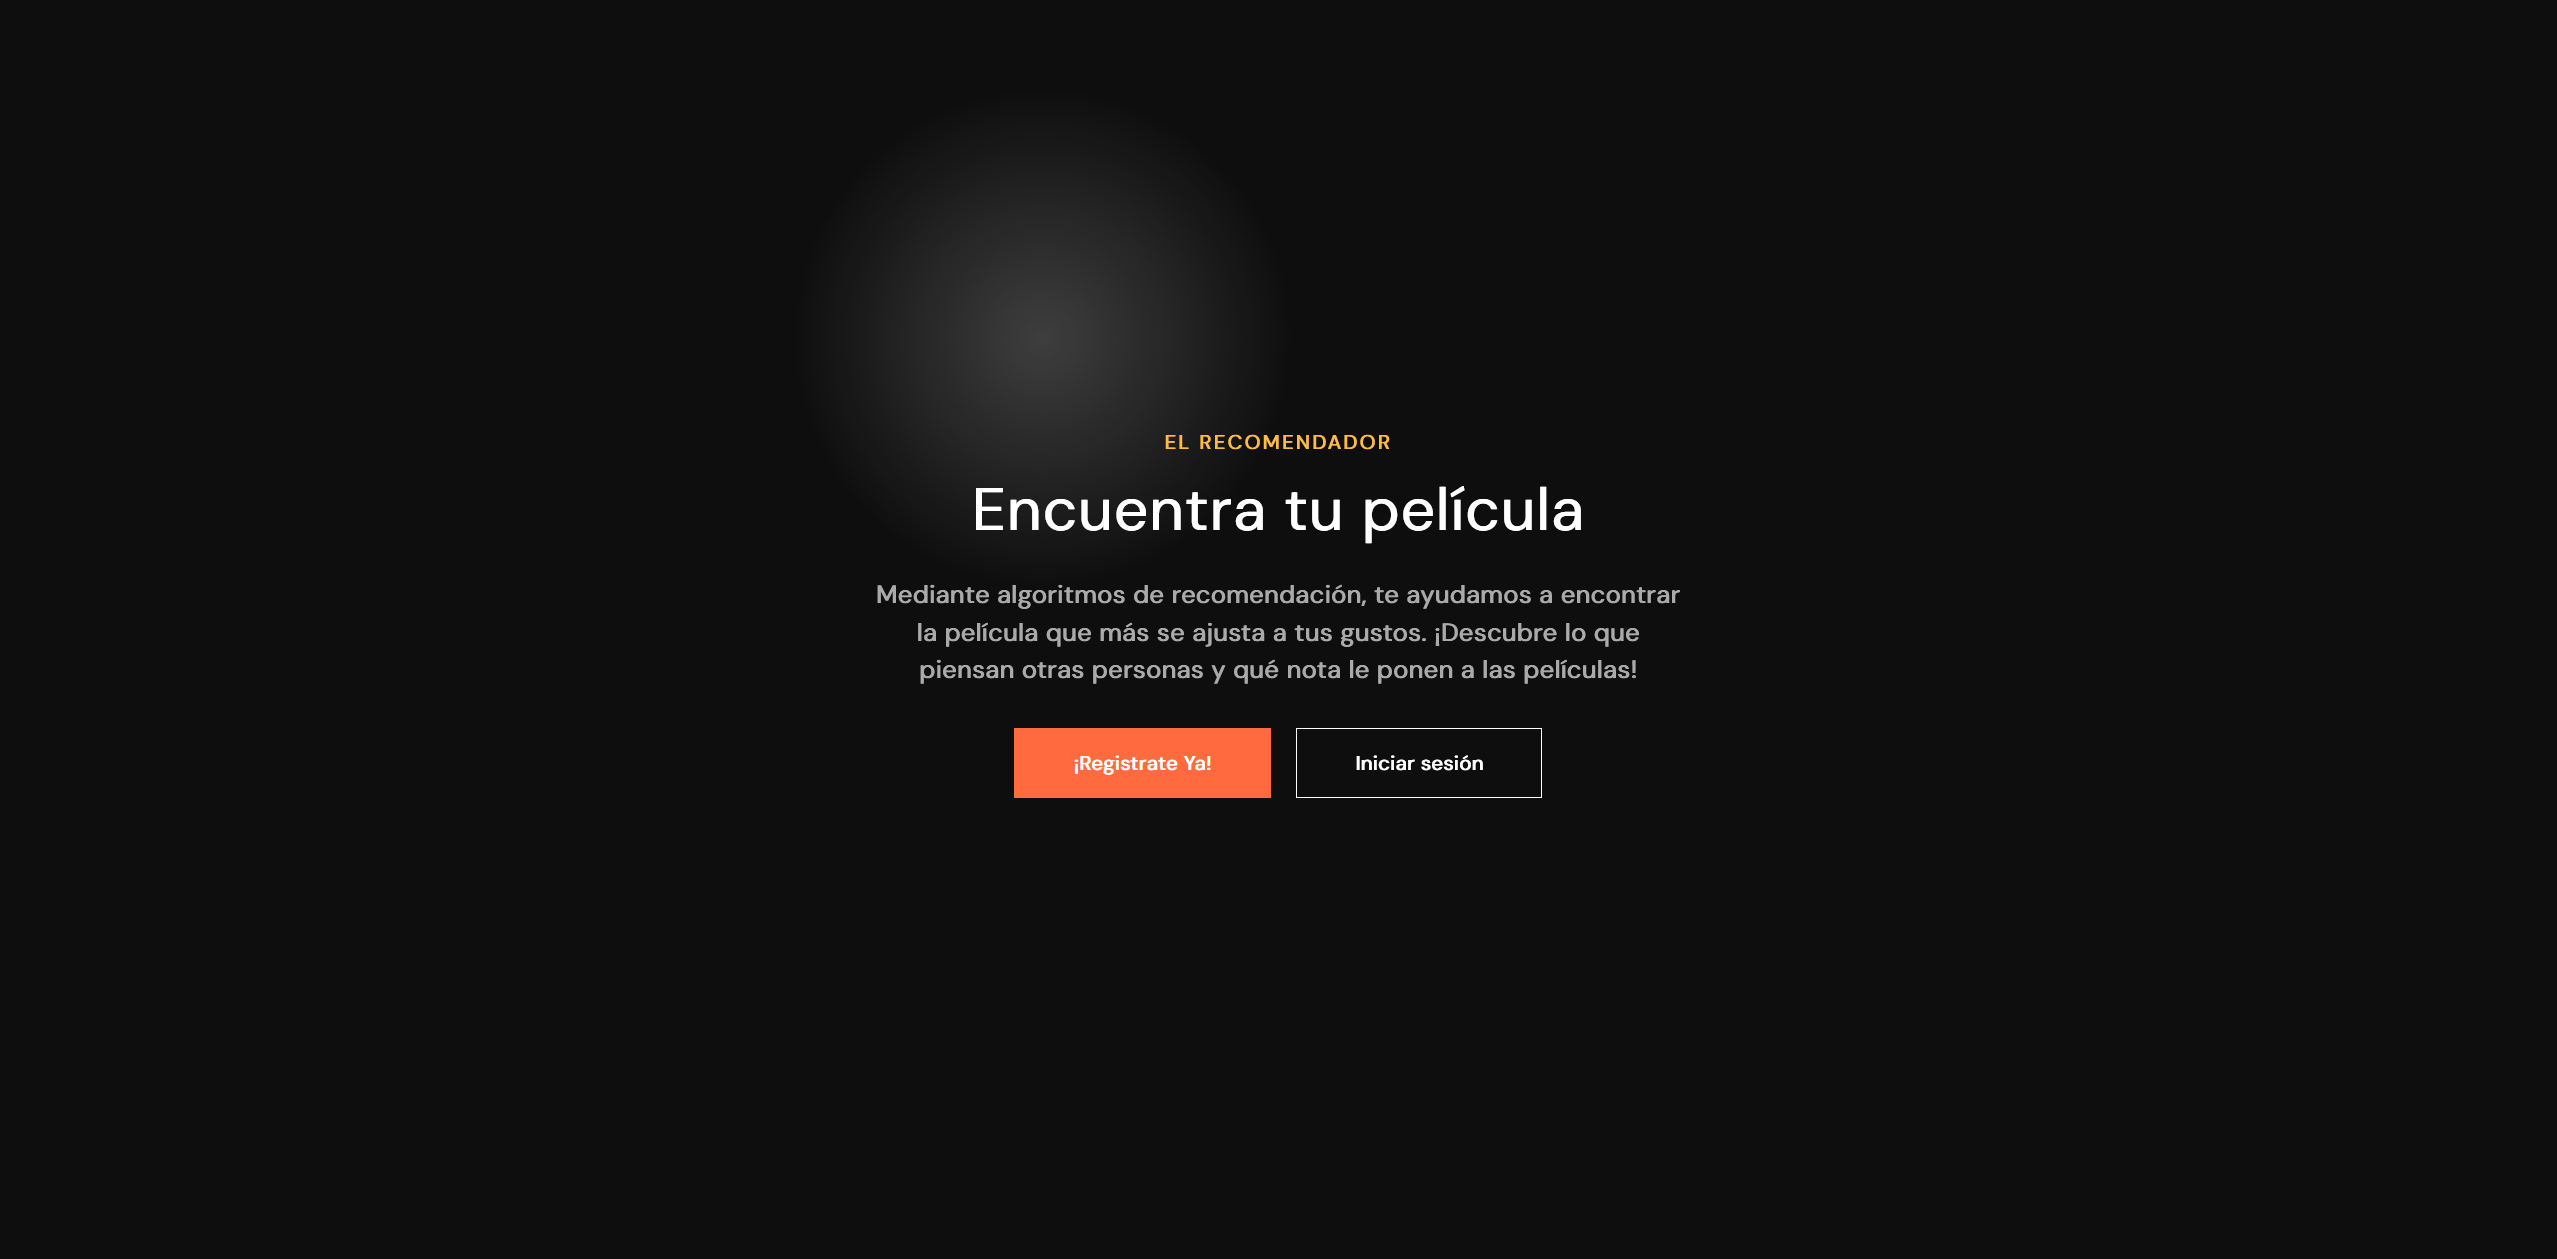
\includegraphics[width=\textwidth]{resources/img/index.png}
            \caption{Inicio de la web.}
            \label{fig:index}
        \end{subfigure}
        \hfill
        \begin{subfigure}{0.45\textwidth}
            
\includegraphics[width=\textwidth]{resources/img/salvapantallasdvd.png}
            \caption{Inspiración del salvapantallas DVD.}
            \label{fig:savescreen}
        \end{subfigure}
        \caption{Comparación entre el index de la web y el salvapantallas DVD.}
        \label{fig:comparacion}
    \end{figure}

    \textit{¿Por qué se ha optado por hacer eso?}

    La razón principal es la posibilidad de implementar un formulario HTML pero que no esté visible al cargar la página, sino que se muestre al hacer clic en el botón correspondiente. La respuesta al botón se realiza mediante \textit{JavaScript}, pero la implementación de dos formulario, con mismo estilo que aparezca como respuesta a un \textit{script}, nos ha llevado a la llamada externa de dichos formularios y que se gestionen por separado en distintos documentos y además a la creación de un archivo de estilos llamado \textit{core.css}, que será un archivo con los estilos comunes a todas las páginas de la web.
    \section{core.css}
    En este archivo podemos encontrar la configuración común a todas las páginas de la web. En él se han definido los estilos de los formularios, las cabeceras, los pie de página, la fuente y el tamaño de la letra...

    Todas las páginas de la web heredarán dichos archivos, y si en alguna página se quiere modificar algún estilo, se puede hacer de forma individual en el archivo de la página correspondiente.

    \begin{figure}[h!]
        \centering
        \begin{subfigure}{0.45\textwidth}
            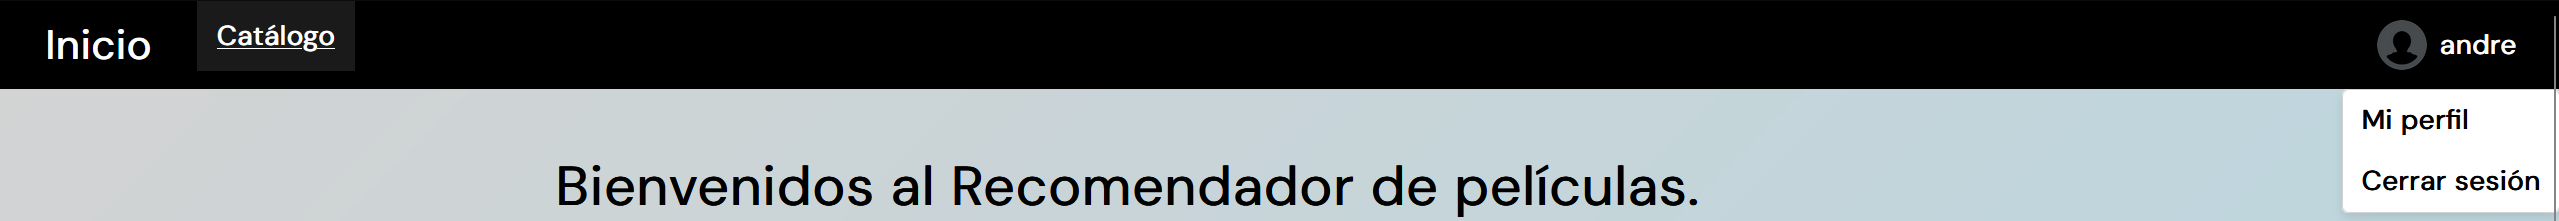
\includegraphics[width=\textwidth]{resources/img/header.png}
            \caption{Header de las páginas.}
            \label{fig:header}
        \end{subfigure}
        \hfill
        \begin{subfigure}{0.45\textwidth}
            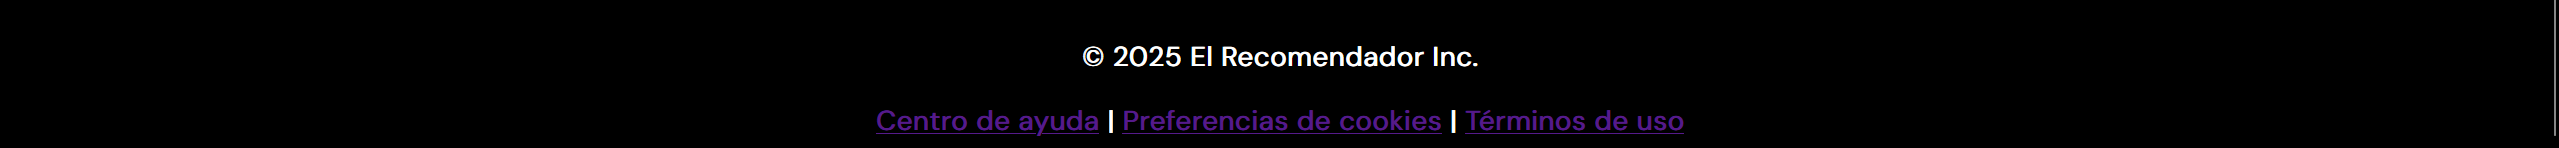
\includegraphics[width=\textwidth]{resources/img/footer.png}
            \caption{Footer de las páginas.}
            \label{fig:footer}
        \end{subfigure}
        \caption{}
        \label{fig:elementoscompartidos}
    \end{figure}

    Un ejemplo claro es la reutilización de recursos como el header y el footer. En la figura~\ref{fig:elementoscompartidos} se puede ver la cabecera y el pie de página de la web. Ambos elementos se han ido utilizando en todas las páginas de la web.

    \chapter{Sección de la autenticación}

    Esta sección trata de la autenticación de los usuarios en la página web. Se encarga de manejar el registro, el
    login y el logout de los usuarios. Además, contiene los archivos necesarios para mantener la sesión activa y de
    verificar que los usuarios estén logueados para acceder a ciertas páginas. Todos estos archivos están en la
    carpeta \textbf{auth} en la raíz del proyecto.

    \section{check\_session.php}

    Esta funcion se encarga de verificar si el usuario está logueado. Tras conectarse a la base de datos, se hará un
    \textbf{query} donde se busque un usuario existente con el id de cookie de la sesión actual. Si no se encuentra,
    será o porque no
    existe la cookie de sesión o porque el usuario no está logueado. En ambos casos, se redirige al usuario a la
    página inicial, el index.html. Si el usuario estaba registrado, se le extiende la cookie una hora. Este archivo
    no tiene HTML, ni salidas, ya que se ejecuta cada vez que una página lo incluye con \textbf{require once}, y
    actuaría como un \textbf{middleware} que protege las páginas de acceso no autorizado sin login.

    \section{loginform.html y registerform.html}

    Estos dos archivos son los formularios de login y registro, respectivamente. Ambos tienen un formulario simple
    con css interno, además de css directo en el html. Son archivos HTML pero sin cabecera ni pie de página, ya que
    lo único que albergan es el formulario en sí, son únicamente un div cada uno, los cuales servirán para hacerle
    \textbf{echo} desde la página de index.html. Esto es para reducir el posible código extenso de html desde los
    archivos login.php y register.php. Ambos formularios tienen un botón de submit que envía los datos mediante una
    petición POST a su respectivo archivo, login.php o register.php.

    \section{login.php y register.php}

    Ambos archivos son los encargados de procesar los datos de los formularios de login y registro, mediante un \textbf{GET}.
    Es decir, según el método de envío de datos procesarán una u otra función. Si reciben una petición GET,
    mostrarán con un echo el formulario:

    \begin{lstlisting}[style=ruled, language=php, caption={Manejo de peticiones GET de login.php y register.php.},
        gobble=4]
    <?php
     if ($_SERVER['REQUEST_METHOD'] === 'GET') {
    echo file_get_contents('loginform.html');
    exit;
        }
    ?>
    \end{lstlisting}

    Si reciben una \textbf{petición POST}, se conectarán a la base de datos y realizarán las consultas
    correspondientes. Para el register, se llamará inicialmente a una función que verifica e inicializa los parámetros de la petición POST,
    teniendo en cuenta que la contraseña tiene un hash \textbf{sha1} y que el id de usuario se suma en 1 al último
    usuario que estaba en esa columna. Luego, se hará un \textbf{query} para insertar el usuario en la base de datos:

    \begin{lstlisting}[style=ruled, language=php, caption={Query de register.php.}, gobble=4]
    <?php
        $query = "INSERT INTO users (id, name, edad, sex, ocupacion, pic, passwd ) VALUES ($params[0], '$params[1]', $params[2], '$params[3]', '$params[4]', '$params[5]', '$params[6]')";
    ?>
    \end{lstlisting}

    Para el login, se hará un \textbf{query} para buscar un usuario con el nombre y la contraseña (previamente
    pasada a la función sha1();) introducidos en el POST.

    \begin{lstlisting}[style=ruled, language=php, caption={Query de login.php.}, gobble=4]
    <?php
        $query = "SELECT * FROM users WHERE name = '$username' AND passwd = '$password'";
    ?>
    \end{lstlisting}

    \section{logout.php}

    A logout.php se le llama varias veces a lo largo del programa para cerrar la sesión, de forma que no hace falta
    reutilizar este código, aunque solo trata de eliminar la cookie restando una hora a la fecha actual.

    \chapter{La carpeta Pages: las páginas visibles}

    La carpeta \textbf{pages}, situada en /textbf{assets/} desde el documentroot, contiene las páginas visibles de la
    web. Estas páginas son las que se mostrarán al usuario con su contenido \textbf{HTML} y \textbf{CSS}. Cada página tiene un archivo \textbf{.php} que se encarga
    de procesar ciertos datos y mostrar la página en sí.

    \section{main.php}

        Es la página principal que se muestra al usuario cuando inicia sesión. Contiene un \textbf{carousel} con las
        primeras películas ordenadas, y debajo estará otro \textbf{carousel} con las películas cargadas del algoritmo.

        Para cargar las películas, como se ha usado la API de \textbf{The Movie Database}, no se podrán cargar todas de
        golpe, por lo que se ha optado por reducir tanto la carga de películas como sus imágenes. Para ello, se hace uso
        del \textbf{lazyload} que carga las imágenes de las películas a medida que se van mostrando en la pantalla, a su
        vez que se van haciendo peticiones asíncronas mediante javascript a la API de TMDB para mostrar la cover de cada película. De este
        modo, se consigue reducir el tiempo de carga de la página y facilitar la navegación al usuario.

    \begin{figure}[H]
        \centering
        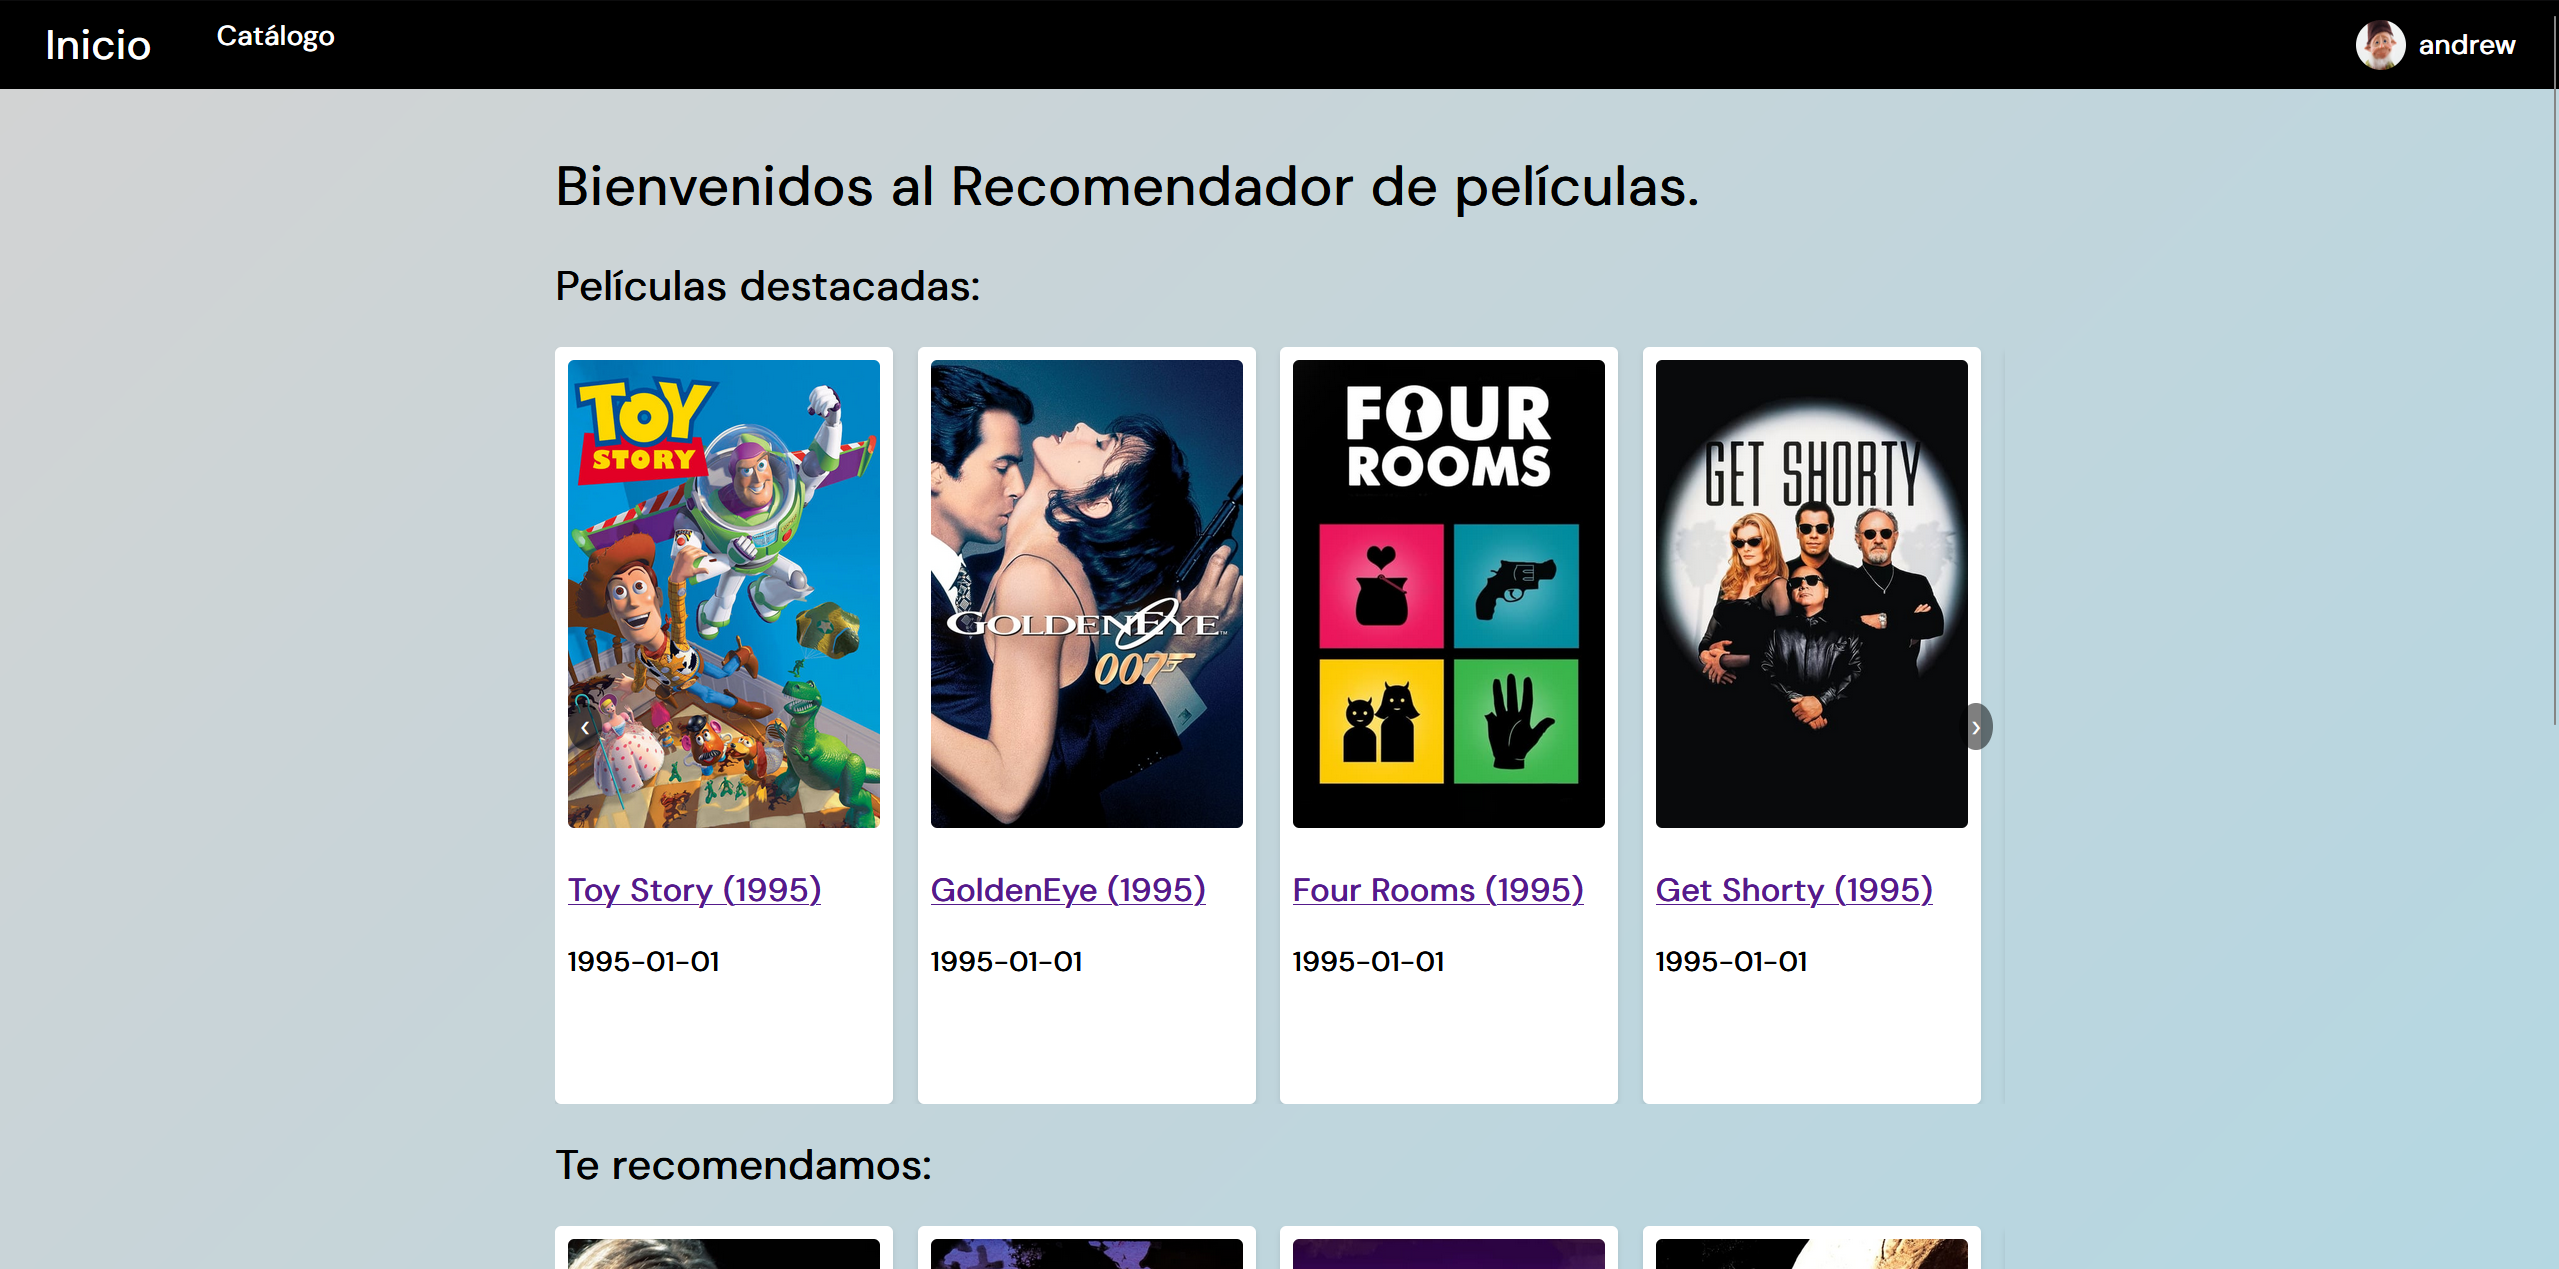
\includegraphics[scale=0.20]{resources/img/main.png}
        \caption{Página main.php.}
        \label{fig:main}
    \end{figure}

    \section{catalog.php}

    La sección del \textbf{catálogo} será similar a la de \textbf{main}, pero en vez de mostrar las películas recomendadas, mostrará todas las películas disponibles en la base de datos filtradas mediante los géneros de éstas. Para ello, se harán distintas peticiones a la base de datos según el género, a su vez de que se podrán ordenar a la vez por título, nombre o puntuación.

    También se realizan peticiones a la base de datos y se procesan en el momento para cargar la media de cada película.

    Todas las películas tienen un enlace a su página de información, donde se se hará un get a \textbf{película.php} con la id.

    \begin{figure}[H]
        \centering
        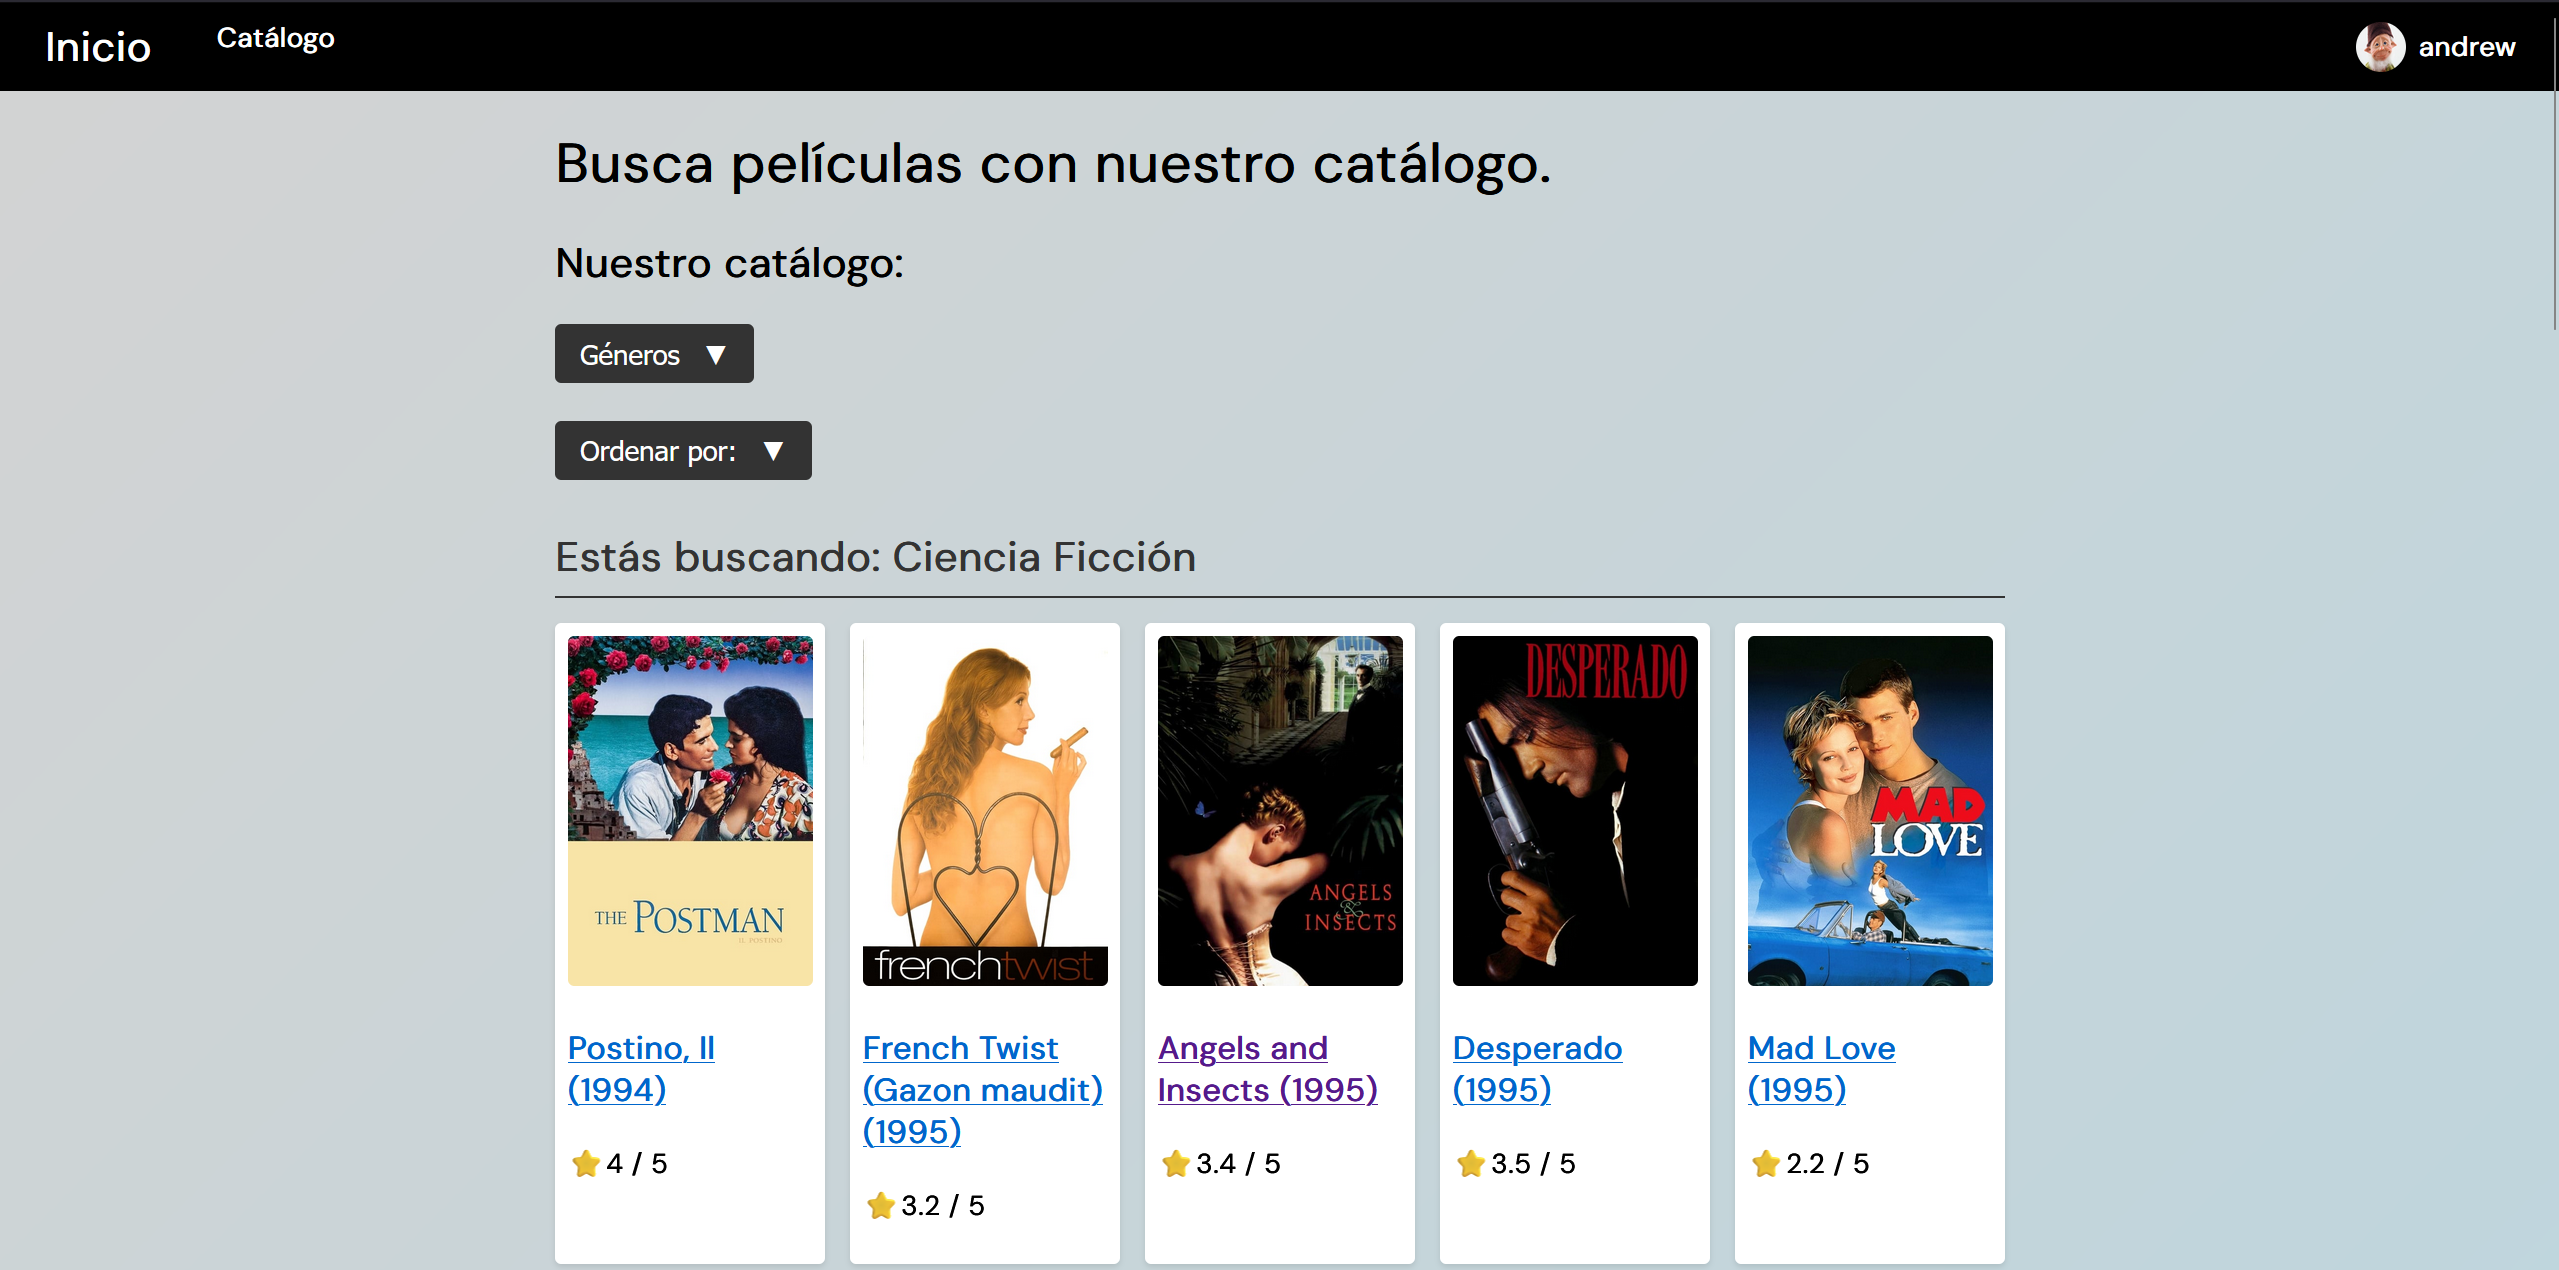
\includegraphics[scale=0.20]{resources/img/catalog.png}
        \caption{Página catalog.php.}
        \label{fig:catalog}
    \end{figure}

    \section{pelicula.php}

    La página de película, al igual que la de perfil, serán como una especie de \textbf{plantilla}, donde recogerá distintas peticiones de la base de datos y las mostrará en la página según la petición GET de la id de la película.

   Se mostrarán datos de la base de datos como la puntuación media y la fecha, a su vez que otros datos aportados por la API de TMDB como el reparto y la duración de la película.

    Además, se mostrarán los comentarios de los usuarios y la posibilidad de puntuar la película, que se gestionan con scripts \textbf{PHP}.

    \begin{figure}[H]
        \centering
        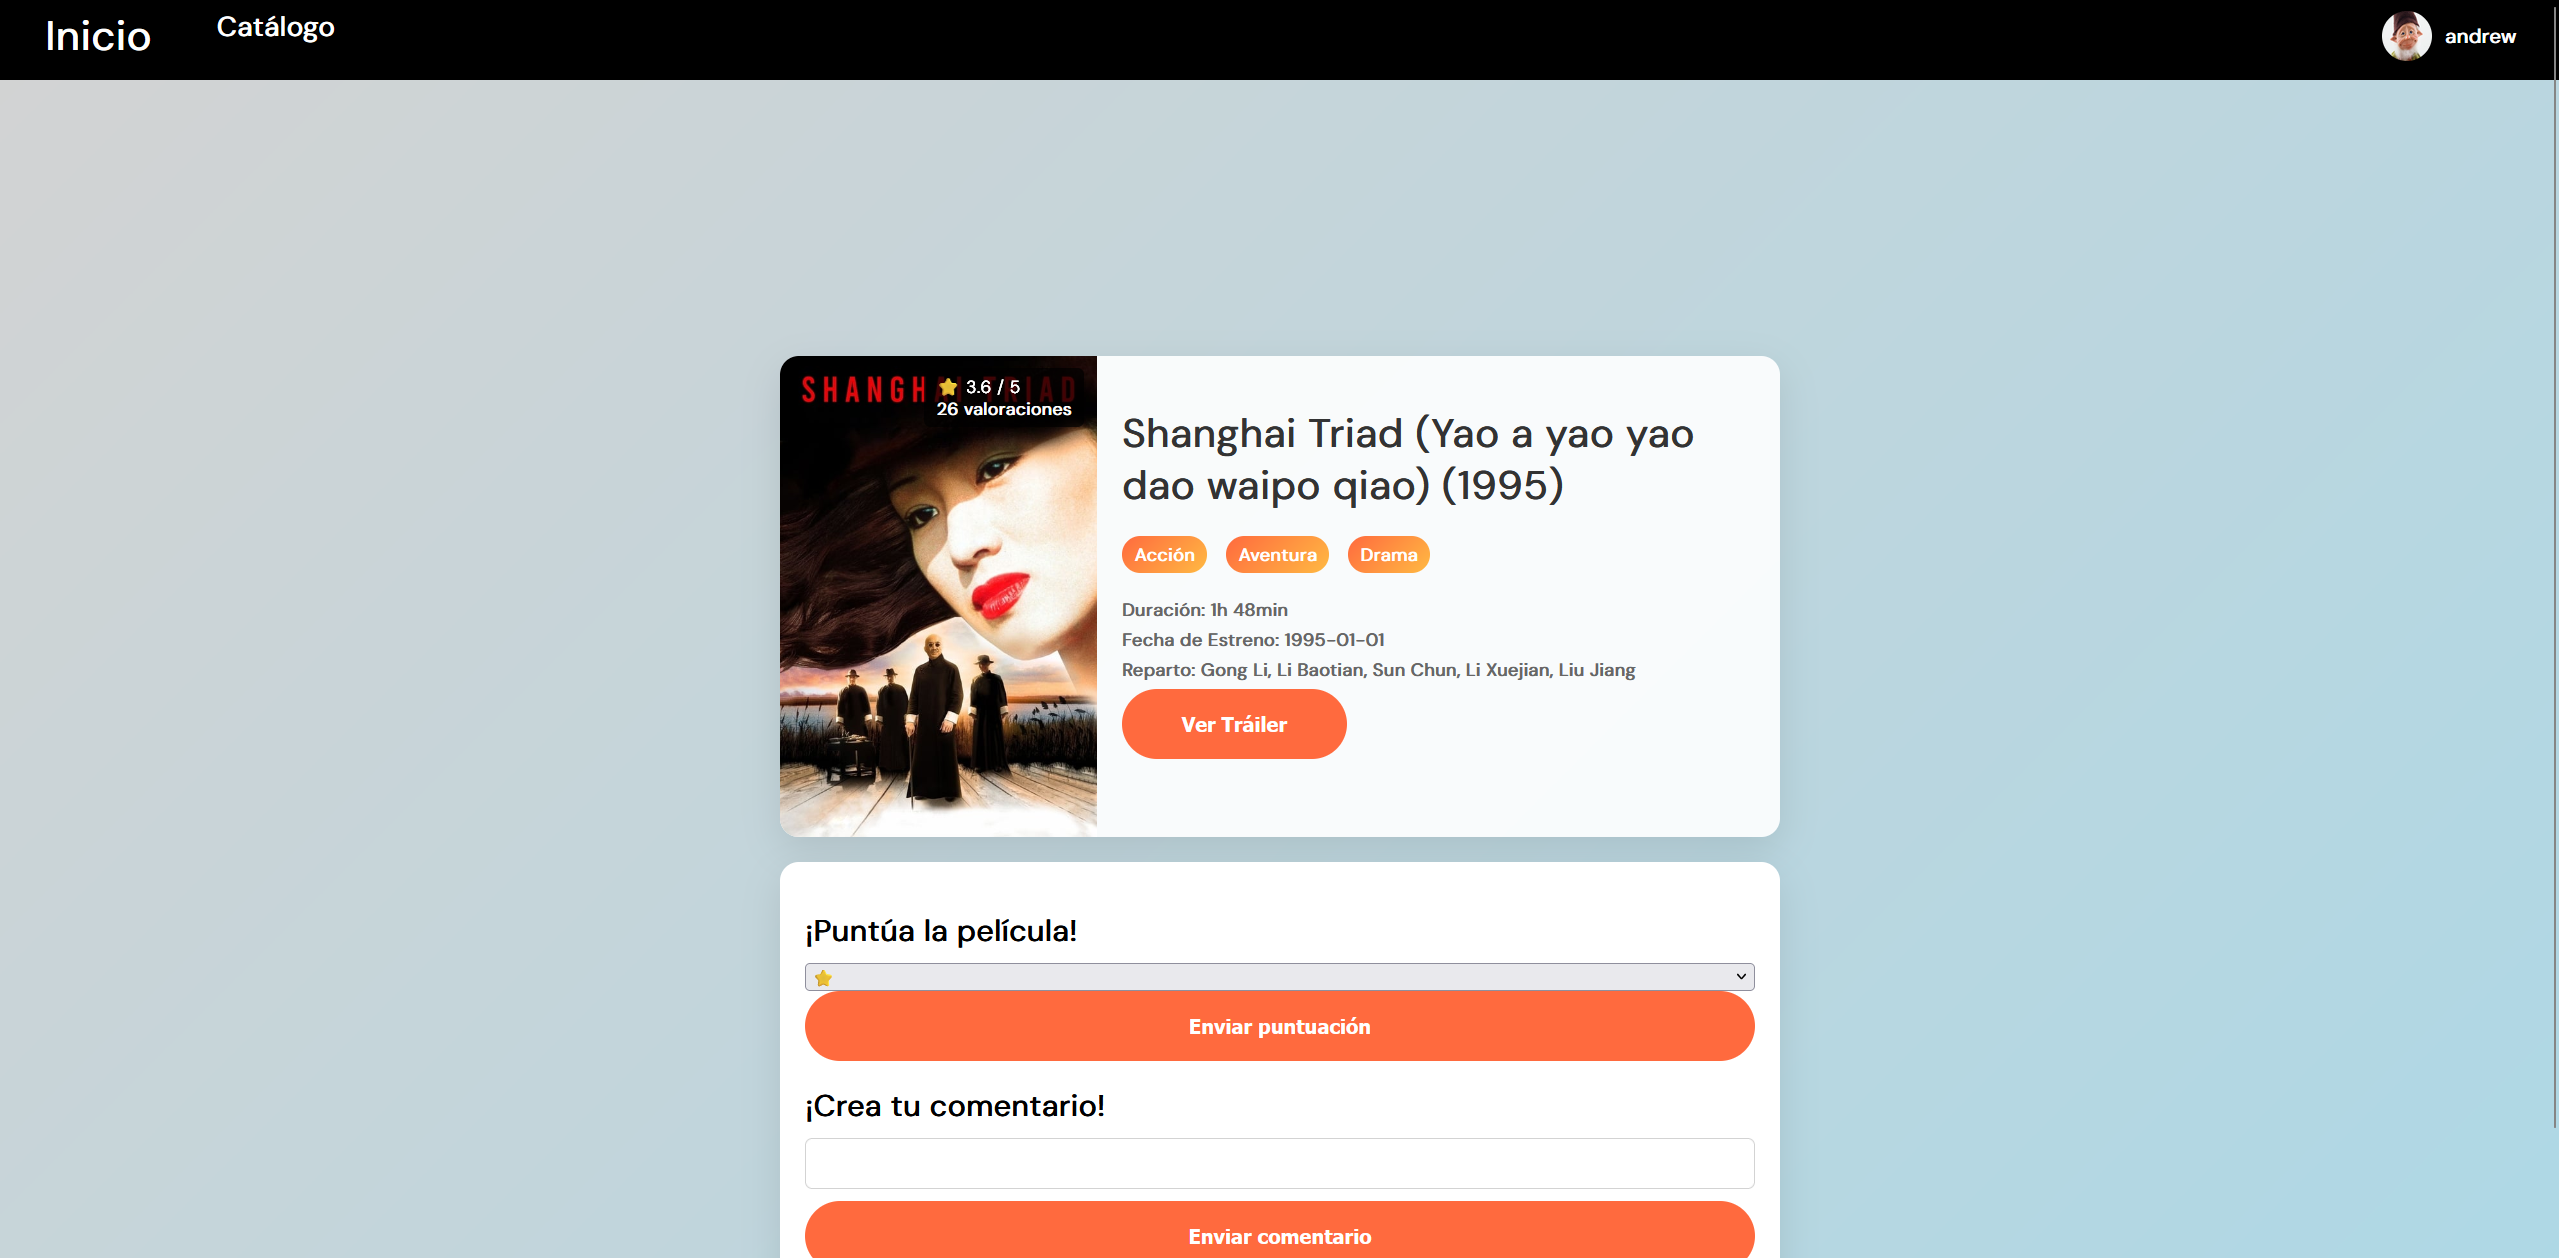
\includegraphics[scale=0.20]{resources/img/movie.png}
        \caption{Página pelicula.php.}
        \label{fig:pelicula}
    \end{figure}
    \section{profile.php}

    En perfil, al igual que en película, será una plantilla que recoja varios datos del usuario según las query que se hacen, decorados con una hoja de estilos. Debajo de los datos, hay un campo para comprobar la contraseña, y el botón de editar perfil, que redirige a \textbf{edit\_profile.php}.

    \begin{figure}[H]
        \centering
        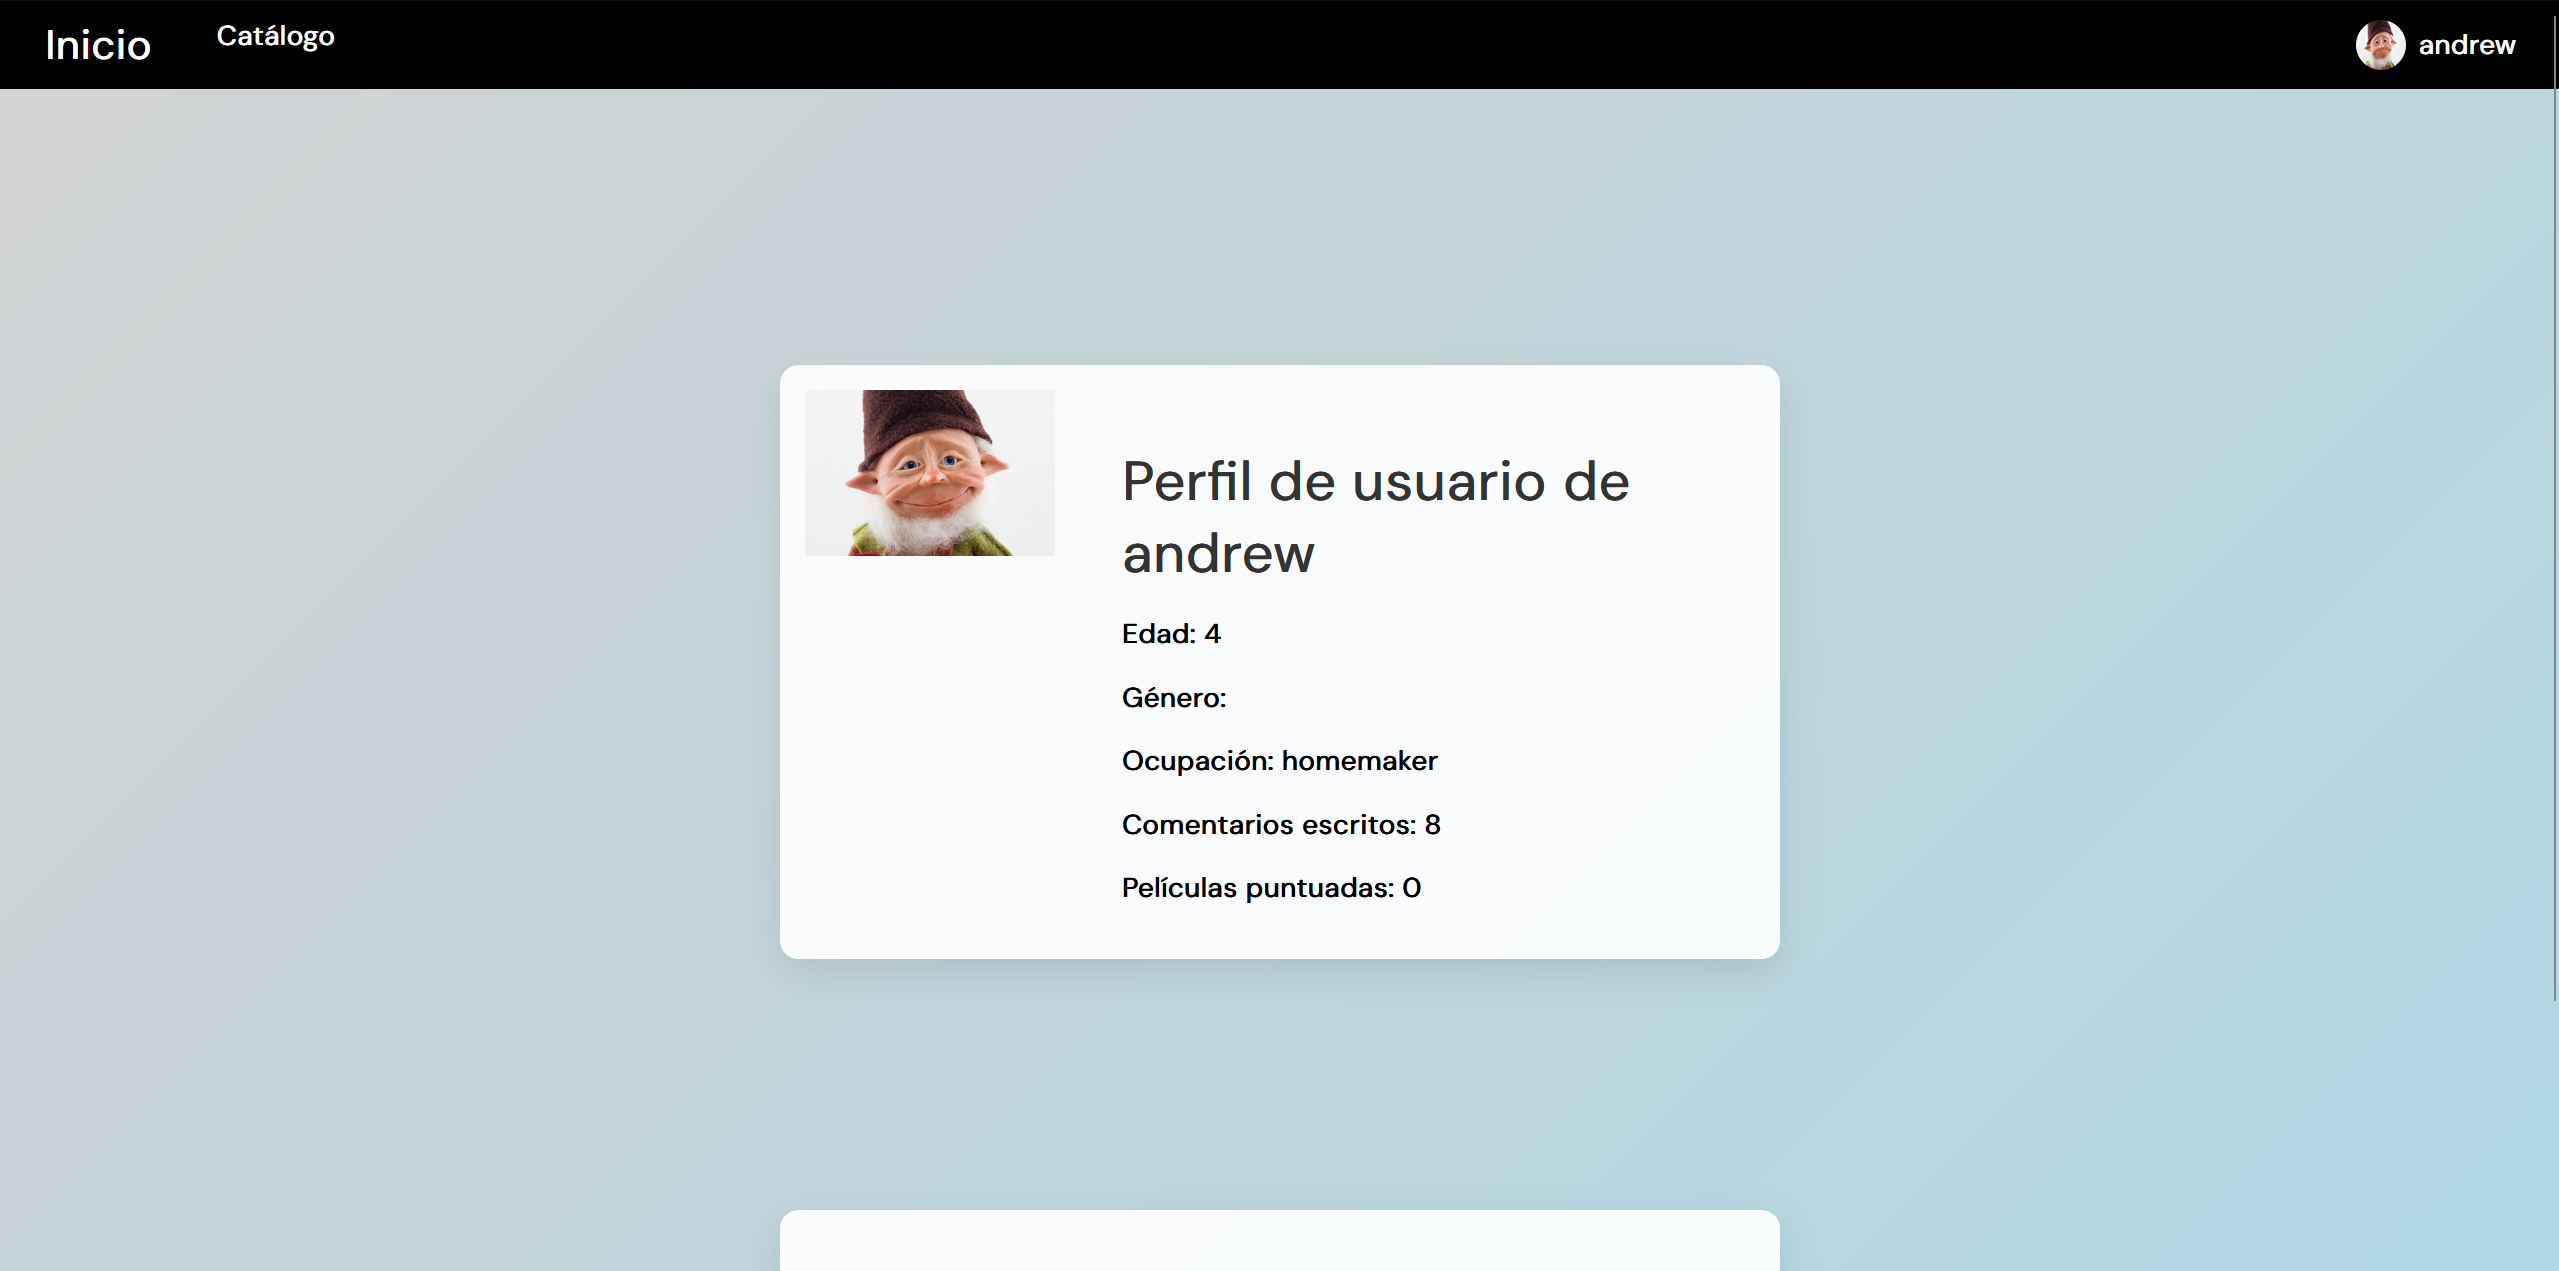
\includegraphics[scale=0.20]{resources/img/profile.png}
        \caption{Página profile.php.}
        \label{fig:profile}
    \end{figure}

    \section{edit\_profile.php}

    En esta página, el usuario podrá editar su perfil, cambiando su nombre, edad, sexo, ocupación y foto de perfil. Para ello, se ha implementado un formulario que actualizará con querys de \textbf{UPDATE} los datos que se han rellenado. Se pueden cambiar por separado, no es necesario todos a la vez. Cabe destacar que la imagen es un campo que únicamente recoge la URL.

    \begin{figure}[H]
        \centering
        \includegraphics[scale=0.20]{resources/img/edit\_profile.png}
        \caption{Página edit\_profile.php.}
        \label{fig:edit}
    \end{figure}

    \chapter{Uso de scripts PHP}

    Estos scripts aparecerán en la carpeta \textbf{php} dentro de \textbf{assets}. Se encargan de procesar varias peticiones GET y POST que se envían desde los archivos anteriores de \textbf{pages}.

    \section{cargar\_comentarios.php}

    Este script se encargará de cargar los comentarios de una película en concreto. Para ello, recibe una petición POST con la id de la película, hace la query correspondiente con los datos necesarios, y devuelve con un formato html, los comentarios y el usuario que los escribe, separados por un br.

    Query de cargar comentarios:
    \begin{lstlisting}[style=ruled, language=php, caption={Query de cargar\_comentarios.php.}, gobble=4]
    <?php
        $query = "SELECT u.name, mc.comment FROM moviecomments mc JOIN users u ON mc.user_id = u.id WHERE mc.movie_id = $movie_id";
    ?>
    \end{lstlisting}


    \section{change\_profile.php}

    Change profile recibirá un POST con los datos a cambiar desde edit\_profile, y actualizará los datos del usuario en la base de datos. Se usa el id del usuario desde la cookie para las query y no se envía en el POST por seguridad.

    \section{check\_password.php}

    Check password recibirá un POST con la contraseña que se quiere comprobar, se hasheará y devolverá un comentario positivo o negativo si coincide con el SHA1 de la contraseña almacenada en la base de datos. Se usa para comprobar la contraseña antes de cambiar el perfil.

    \section{crear\_comentario.php}

    Crear comentario recibirá un POST con el id de la película y el comentario a insertar. Se insertará en la base de datos con el id del usuario y el id de la película, que también se recibe en el POST.

    \section{puntuar\_pelicula.php}

    Similar a crear comentario, pero en vez de insertar un comentario, se insertará una puntuación. Se recibirá un POST con el id de la película y la puntuación, y se insertará en la base de datos con el id del usuario y el id de la película.

    Ambos redirigen a la página de la película con la id de la película en la que se estaba para similar mayor dinamismo.

    \chapter{Includes}
    Se ha decidido crear un directorio \textit{includes} la cual contenga scripts PHP que se van a utilizar en varias páginas de la web. De esta forma, se evita la repetición de código y se facilita la gestión de los mismos.
    \section{common.php}
    Este script se encarga principalmente de recolectar toda la información para las películas, desde llamadas a API hasta consulta de base de datos de las puntuaciones de cada película.
    \section{conectar.php}
    Se centraliza la conexión a la base de datos en este script. De esta forma, se evita la repetición de código y haciendolo más legible.
    \section{genres.php}
    Consulta a la base de datos de información de los géneros para una película \textit{i}.
    \section{movies.php}
    Realiza una consulta paginada a una base de datos para obtener una lista de películas, opcionalmente filtradas por género, y devuelve los resultados en formato JSON.

    \chapter{JavaScript}

    Los scripts de \textit{JavaScript} tiene una implementación variada, nos podemos encontar desde scripts sencillos para el index.html~\ref{fig:comparacion} hasta scripts combinados para poder cargar de forma asíncrona las imágenes de las peliculas.

    \section{carousel.js}
    Aunque nos hubiese gustado crear una implementación completa (scroll vertical "aparentemente infinto" y el carousel \cite{carousel}),
    \section{dropdownLogout.js}
    DropdownLogout es un scprit sencillo que se encarga de escuchar el click en el nombre de usuario para desplegar 2 botones, "Cerrar sesión" y "Mi perfil".
    \section{lazyload.js}
    Para la carga de imágenes, nos hemos enfrentado a un problema crucial y es que la página no se quede colgada durante largos segundos hasta que la carga de todas las imágenes se complete, para ello hemos decidido implementar \textit{Lazy Loading}\cite{lazyloading}. Con ello solucionamos todos los problemas de carga de imágenes y la página funciona desde el instante 0 sin necesidad de que carguen todas las imágenes.
    \section{main.js}
    Este script sólo se encarga de la parte estética del \textit{index.html}, haciendo que la "luz" rebote contra los bordes de la ventana.

    \chapter{Matlab y los algoritmos}
    Los algoritmos en Matlab se han implementado desde la carpeta \textit{matlab}. En ella se encuentran los archivos \textit{getData.m} y \textit{updateRecommendation.m} entre otros, que son los encargados de la conexión con la base de datos y de la actualización de las recomendaciones, respectivamente.
    Cabe recalcar que no se ha podido comprobar el funcionamiento de los algoritmos y su correcta implementación en la web, ya que no se ha podido correr un servidor de Matlab en la máquina local no tampoco del servidor ofrecido para la entrega.
    \section{Conexión BBDD con Matlab}
    La conexión a la base de datos se gestiona medinante 2 archivos, \textit{getData.m} ofrecido por el profesor, y \textit{updateRecommendation.m} . Todos esos datos son los que nos permiten procesar la información y realizar las recomendaciones.
    \section{main.m}
    En este archivo se centraliza toda la lógica de los algoritmos de recomendación y la puntuación Bayesiana. Recoge los datos necesarios y realiza las iteraciones necesarias para obtener los resultados. Posteriormente esos datos son enviados a la base de datos.
    \section{Algoritmo de puntaje con Bayesian Ranking}
    Para realizar el puntuaje con Bayesian Ranking, se ha utilizado la siguiente fórmula:
    \begin{equation}
        p_i = \frac{NR+n_ir_i}{N+n_i}
    \end{equation}    siendo $N$ el número total de películas, $R$ la puntuación media de todas las películas, $n_i$ el número de puntuaciones de la película $i$, $r_i$ la puntuación media de la película $i$, $m$ la puntuación media de todas las películas y $v$ la varianza de las puntuaciones de todas las películas.
    \newpage


    %%%%%%%%%%%%%%%%%%%%%%%%%%%%%%%%%%%%%%%%%%%%%%%%%%%%%%%%%%%%%%%%%%%%%%%%%%%%%%%%%%%%%%%%%%%%
    % ------------------TODO LO QUE ESTÁ ABAJO HAY QUE ELIMINARLO LUEGO----------------------- %
    %%%%%%%%%%%%%%%%%%%%%%%%%%%%%%%%%%%%%%%%%%%%%%%%%%%%%%%%%%%%%%%%%%%%%%%%%%%%%%%%%%%%%%%%%%%%
    \printbibliography

\end{document}
